I tipi di interfaccia esprimono generalizzazioni o astrazioni sui comportamenti di altri tipi.
Generalizzando, le interfacce ci permettono di scrivere funzioni più flessibili e adattabili perché non sono legate ai dettagli di una particolare implementazione.

Ciò che rende le interfacce di Go così distintive è che sono \textit{soddisfatte implicitamente}.
In altre parole, non c'è bisogno di dichiarare tutte le interfacce che un dato tipo concreto soddisfa;
basta semplicemente possedere i metodi necessari.
Questo design consente di creare nuove interfacce che sono soddisfatte dai tipi concreti esistenti senza modificare i tipi esistenti, il che è particolarmente utile per i tipi definiti in pacchetti che non si controllano.


\section{Interfacce come contratti}
\label{sec:interfacce_come_contratti}%
Tutti i tipi esaminati finora sono stati \textit{tipi concreti}.
Un tipo concreto specifica la rappresentazione esatta dei suoi valori ed espone le operazioni intrinseche di tale rappresentazione, come l'aritmetica per i numeri, o l'indicizzazione, l'\verb|append| e il \verb|range| per le slice.
Un tipo concreto può anche fornire comportamenti aggiuntivi attraverso i suoi metodi.
Quando si ha un valore di tipo concreto, si sa esattamente di cosa \textit{si tratta} e cosa \textit{si può fare} con esso.

C'è un'altra tipologia di tipi in Go chiamata \textit{interfaccia}.
L'interfaccia è un \textit{tipo astratto}.
Essa non espone all'esterno la sua struttura interna e quella dei suoi valori e non rivela l'insieme base di operazioni che questi valori supportano;
solo alcuni metodi sono visibili all'esterno.
Quando si ha un valore di un tipo interfaccia, non si sa nulla di ciò che \textit{è};
si sa solo cosa può \textit{fare}, o più precisamente, i comportamenti che i suoi metodi forniscono.

Ci sono due funzioni simili per la formattazione delle stringhe: \verb|fmt.Printf|, che scrive il risultato sullo standard output (un file), e \verb|fmt.Sprintf|, che restituisce il risultato come una \verb|string|.
Sarebbe un peccato se la parte difficile, formattare il risultato, dovesse essere duplicata a causa di queste differenze superficiali nel modo in cui il risultato viene utilizzato.
Grazie alle interfacce, non succede.
Entrambe queste funzioni sono, in effetti, wrapper intorno a una terza funzione, \verb|fmt.Fprintf|, che è agnostica su ciò che accade al risultato che calcola:
\begin{lstlisting}[frame=single, label={lst:lstlisting6-1.1}]
package fmt

func Fprintf(w io.Writer, format string,
    args ...interface{}) (int, error)

func Printf(format string, args ...interface{}) (int, error) {
    return Fprintf(os.Stdout, format, args...)
}

func Sprintf(format string, args ...interface{}) string {
    var buf bytes.Buffer
    Fprintf(&buf, format, args...)
    return buf.String()
}
\end{lstlisting}
Il prefisso \verb|F| di \verb|Fprintf| sta per \textit{file} e indica che l'output formattato dovrebbe essere scritto nel file fornito come primo argomento.
Nel caso di \verb|Printf|, l'argomento, \verb|os.Stdout|, è un \verb|*os.file|.
Nel caso di \verb|Sprintf|, tuttavia, l'argomento non è un file, anche se superficialmente può somigliare: \verb|&buf| è un puntatore a un buffer di memoria in cui i byte possono essere scritti.

Il primo parametro di \verb|Fprintf| non è nemmeno un file.
È un \verb|io.Writer|, che è un tipo di interfaccia con la seguente dichiarazione:
\begin{lstlisting}[frame=single, label={lst:lstlisting6-1.2}]
package io

// Writer is the interface that wraps the basic Write method.
type Writer interface {
    // Write writes len(p) bytes from p to the underlying
    // data stream. It returns the number of bytes written from
    // p (0 <= n <= len(p)) and any error encountered that
    // caused the write to stop early. Write must return a
    // non-nil error if it returns n < len(p). Write must not
    // modify the slice data, even temporarily.
    //
    // Implementations must not retain p.
    Write(p []byte) (n int, err error)
}
\end{lstlisting}
L'interfaccia \verb|io.Writer| definisce il contratto tra \verb|Fprintf| e i suoi chiamanti.
Da un lato, il contratto richiede che il chiamante fornisca un valore di un tipo concreto come \verb|*os.File| o \verb|*bytes.Buffer| che ha un metodo chiamato \verb|Write| con la firma e il comportamento appropriati.
D'altra parte, il contratto garantisce che \verb|Fprintf| farà il suo lavoro dato qualsiasi valore che soddisfi l'interfaccia \verb|io.Writer|.
\verb|Fprintf| non può presumere che stia scrivendo su un file o una memoria, solo che possa chiamare \verb|Write|.

Si può tranquillamente passare un valore di qualsiasi tipo concreto che soddisfi \verb|io.Writer| come primo argomento a \verb|fmt.Fprintf|.
Questa libertà di sostituire un tipo con un altro che soddisfi la stessa interfaccia è chiamata \textit{sostituibilità} ed è un segno distintivo della programmazione orientata agli oggetti.

Viene presentato ora un esempio di tipo concreto che soddisfa l'interfaccia \verb|io.Writer|.
Il metodo di scrittura del tipo \verb|*ByteCounter| conta soltanto i byte scritti prima di scartarli.
\begin{lstlisting}[frame=single, label={lst:lstlisting6-1.3}]
type ByteCounter int

func (c *ByteCounter) Write(p []byte) (int, error) {
    *c += ByteCounter(len(p)) // converte int in ByteCounter
    return len(p), nil
}
\end{lstlisting}
Poiché \verb|*ByteCounter| soddisfa il contratto di \verb|io.Writer|, lo si può passare in input a \verb|Fprintf|, che fa la sua formattazione stringa ignaro di questo cambiamento;
il \verb|ByteCounter| accumula correttamente la lunghezza del risultato.
\begin{lstlisting}[frame=single, label={lst:lstlisting6-1.4}]
var c ByteCounter
c.Write([]byte(%*``*\)hello%*''*\)))
fmt.Println(c)

c = 0 // reset del contatore
var name = %*``*\)Dolly%*''*\)
fmt.Fprintf(&c, %*``*\)hello, %s%*''*\), name)
fmt.Println(c)
\end{lstlisting}
Output:
\begin{lstlisting}[language=bash, frame=L, label={lst:lstlisting6-1.5}]
5
12
\end{lstlisting}
Oltre a \verb|io.Writer|, c'è un'altra interfaccia di grande importanza per il package \verb|fmt|.
\verb|Fprintf| e \verb|Fprintln| forniscono un modo per i tipi di controllare come vengono stampati i loro valori.
Dichiarare un metodo \verb|String| rende un tipo capace di soddisfare una delle interfacce più utilizzate di tutti, \verb|fmt.Stringer|:
\begin{lstlisting}[frame=single, label={lst:lstlisting6-1.6}]
package fmt

// The String method is used to print values passed
// as an operand to any format that accepts a string
// or to an unformatted printer such as Print.
type Stringer interface {
    String() string
}
\end{lstlisting}


\section{Tipi di interfaccia}
\label{sec:tipi_di_interfaccia}%
Un tipo di interfaccia specifica un insieme di metodi che un tipo concreto deve possedere per essere considerato un'istanza di quell'interfaccia.

Un \verb|Reader| rappresenta qualsiasi tipo da cui è possibile leggere byte e un \verb|Closer| un qualsiasi valore che è possibile chiudere, come un file o una connessione di rete.
\begin{lstlisting}[frame=single, label={lst:lstlisting6-2.1}]
package io

type Reader interface {
    Read(p []byte) (n int, err error)
}

type Closer interface {
    Close() error
}
\end{lstlisting}
Si trovano anche dichiarazioni di nuovi tipi di interfaccia come combinazioni di quelli esistenti.
\begin{lstlisting}[frame=single, label={lst:lstlisting6-2.2}]
type ReadWriter interface {
    Reader
    Writer
}

type ReadWriteCloser interface {
    Reader
    Writer
    Closer
}
\end{lstlisting}
La sintassi usata sopra, che assomiglia all'embedding di struct, permette di definire un'altra interfaccia senza dover scrivere tutti i suoi metodi.
Questa operazione è detta \textit{embedding} di un'interfaccia.
Si poteva anche scrivere l'interfaccia \verb|io.ReadWriter| senza fare l'embedding, anche se in modo meno succinto, in questo modo:
\begin{lstlisting}[frame=single, label={lst:lstlisting6-2.3}]
type ReadWriter interface {
    Read(p []byte) (n int, err error)
    Write(p []byte) (n int, err error)
}
\end{lstlisting}
o anche utilizzando un mix dei due stili:
\begin{lstlisting}[frame=single, label={lst:lstlisting6-2.4}]
type ReadWriter interface {
    Read(p []byte) (n int, err error)
    Writer
}
\end{lstlisting}
L'ordine in cui appaiono i metodi è irrilevante.
Tutto ciò che conta è l'insieme dei metodi.


\section{Soddisfacimento dell'interfaccia}
\label{sec:soddisfacimento_interfaccia}%
Un tipo \textit{soddisfa} un'interfaccia se possiede tutti i metodi che l'interfaccia richiede.

La regola di assegnabilità per le interfacce è molto semplice: un'espressione può essere assegnata a un'interfaccia solo se il suo tipo soddisfa l'interfaccia.
\begin{lstlisting}[frame=single, label={lst:lstlisting6-3.1}]
var w io.Writer
w = os.Stdout         // OK: *os.File ha il metodo Write
w = new(bytes.Buffer) // OK: *bytes.Buffer ha il metodo Write
w = time.Second       // compile error: time.Duration non ha il
                      // metodo Write

var rwc io.ReadWriteCloser
rwc = os.Stdout         // OK: *os.File ha i metodi Read, Write,
                        // Close
rwc = new(bytes.Buffer) // compile error: *bytes.Buffer non ha
                        // il metodo Close
\end{lstlisting}
La regola si applica anche quando il lato destro è esso stesso un'interfaccia:
\begin{lstlisting}[frame=single, label={lst:lstlisting6-3.2}]
w = rwc // OK: io.ReadWriteCloser ha il metodo Write
rwc = w // compile error: io.Writer non ha il metodo Close
\end{lstlisting}
Il tipo \verb|interface{}|, detto \textit{interfaccia vuota}, è indispensabile.
Poiché il tipo di interfaccia vuota non pone richieste sui tipi che lo soddisfano, possiamo assegnare \textit{qualsiasi} valore all'interfaccia vuota.
\begin{lstlisting}[frame=single, label={lst:lstlisting6-3.3}]
var any interface{}
any = true
any = 12.34
any = %*``*\)hello%*''*\)
any = map[string]int{%*``*\)one%*''*\): 1}
any = new(bytes.Buffer)
\end{lstlisting}
Naturalmente, avendo creato un \verb|interface{}| contenente un valore booleano, float, string, map, puntatore, o qualsiasi altro tipo, non è possibile far nulla direttamente al valore che detiene poiché l'interfaccia non ha metodi.

Poiché il soddisfacimento dell'interfaccia dipende solo dai metodi dei due tipi coinvolti, non è necessario dichiarare la relazione tra un tipo concreto e le interfacce che soddisfa.

Tipi di interfaccia non vuoti come \verb|io.Writer| sono più spesso soddisfatti da un tipo di puntatore, in particolare quando uno o più dei metodi di interfaccia implica una sorta di mutazione al ricevitore, come fa il metodo \verb|Write|.
Un puntatore a una struttura è un tipo di metodo particolarmente comune.

Ma i tipi di puntatore non sono affatto gli unici tipi che soddisfano le interfacce, e anche le interfacce con i metodi mutatore possono essere soddisfatte da uno degli altri tipi di riferimento di Go.

Un tipo concreto può soddisfare molte interfacce non correlate.
Immaginiamo di avere un programma che organizza o vende manufatti culturali digitalizzati come musica, film e libri.
Si potrebbe definire la seguente serie di tipi concreti:
\begin{lstlisting}[frame=single, label={lst:lstlisting6-3.4}]
Album
Book
Movie
Magazine
Podcast
TVEpisode
Track
\end{lstlisting}
Possiamo esprimere ogni astrazione di interesse come un'interfaccia.
Alcune proprietà sono comuni a tutti gli artefatti, come il titolo, la data di creazione e la lista dei creatori (autori e artisti).
\begin{lstlisting}[frame=single, label={lst:lstlisting6-3.5}]
type Artifact interface {
    Title() string
    Creators() []string
    Created() time.Time
}
\end{lstlisting}
Le altre proprietà sono ristrette ad alcuni dei tipi di artefatti.
La prioprietà relative ai testi stampati sono rilevanti solo ai libri e ai magazine, mentre solo i film e gli episodi televisivi hanno la proprietà della risoluzione dello schermo.
\begin{lstlisting}[frame=single, label={lst:lstlisting6-3.6}]
types Text interface {
    Pages() int
    Words() int
    PageSize() int
}

type Audio interface {
    Stream() (io.ReadCloser, error)
    RunningTime() time.Duration
    Format() string // p.e., %*\textit{``}*\)MP3%*\textit{''}*\), %*\textit{``}*\)WAV%*\textit{''}*\)
}

type Video interface {
    Stream() (io.ReadCloser, error)
    RunningTime() time.Duration
    Format() string // p.e., %*\textit{``}*\)MP4%*\textit{''}*\), %*\textit{``}*\)WMV%*\textit{''}*\)
    Resolution() (x, y int)
}
\end{lstlisting}
Queste interfacce permettono di aggregare tipi concreti e di esprimere gli aspetti che condividono.
Per esempio, se bisogna gestire gli oggetti \verb|Audio| e \verb|Video| allo stesso modo, si può definire un'interfaccia \verb|Streamer| per rappresentare gli aspetti che hanno in comune senza cambiare alcun tipo dichiarato già esistente.
\begin{lstlisting}[frame=single, label={lst:lstlisting6-3.7}]
type Streamer interface {
    Stream() (io.ReadCloser, error)
    RunningTime() time.Duration
    Format() string
}
\end{lstlisting}
Ogni gruppo di tipi concreti che si basano sui loro comportamenti condivisi possono essere espressi come un tipo di interfaccia.
A differenza dei linguaggi fondati sulle classi, dove l'insieme delle classi che soddisfano le interfacce è esplicito, in Go si può definire una nuova astrazione o gruppi di interesse quando diventa necessario, senza andare a modificare le dichiarazioni dei tipi concreti.
Questo è particolarmente utile quando il tipo concreto sta in un package scritto da un programmatore terzo.


\section{Parsing Flags con flag.Value}
\label{sec:parsing_flags_con_flagvalue}%
L'interfaccia standard \verb|flag.Value| aiuta a definire una nuova notazione per i flag da linea di comando.
Si consideri il seguente programma che si sospende per un periodo di tempo.
\begin{lstlisting}[frame=single, label={lst:lstlisting6-4.1}]
var period = flag.Duration(%*``*\)period%*''*\), 1*time.Second,
    %*``*\)sleep period%*''*\))

func main() {
    flag.Parse()
    fmt.Printf(%*``*\)Sleeping for %v...%*''*\), *period)
    time.Sleep(*period)
    fmt.Println()
}
\end{lstlisting}
Prima di sospendersi il main stampa il periodo di tempo.
Il package \verb|fmt| chiama il metodo \verb|String| di \verb|time.Duration| a stampare il periodo di tempo in formato di secondi, ma con una notazione user-friendly:
\begin{lstlisting}[language=bash, frame=L, label={lst:lstlisting6-4.2}]
$ go build sleep
$ ./sleep
Sleeping for 1s...
\end{lstlisting}
Di default, il periodo di sospensione è di un secondo, ma può essere cambiato tramite il flag da linea di comando \verb|-period|.
La funzione \verb|flag.Duration| crea una variabile flag di tipo \verb|time.Duration| e permette all'utente di specificare la durata nel formato che più preferisce l'utente, incluso la stessa notazione stampata dal metodo \verb|String|.
Quesa simmetria di design porta ad un'interfaccia utente ordinata.
\begin{lstlisting}[language=bash, frame=L, label={lst:lstlisting6-4.3}]
$ ./sleep -period 50ms
Sleeping for 50ms...
$ ./sleep -period 2m30s
Sleeping for 2m30s...
$ ./sleep -period 1.5h
Sleeping for 1h30m0s...
$ ./sleep -period %*``*\)1 day%*''*\)
inval value %*``*\)1 day%*''*\) for flag -period: time: invalid duration 1
day
\end{lstlisting}
Proprio grazie all'utilità dei valori di durata dei flag, questa funzionalità è definita all'interno del package \verb|flag|, ma è semplice definire una nuova notazione di un flag per il proprio tipo di dati.
Bisogna solo definire un tipo che soddisfi l'interfaccia \verb|flag.Value|, che ha la seguente dichiarazione:
\begin{lstlisting}[frame=single, label={lst:lstlisting6-4.4}]
package flag

// Value is the interface to the value stored in a flag.
type Value interface {
    String() string
    Set(string) error
}
\end{lstlisting}
Il metodo \verb|String| formatta il valore del flag per un uso da linea di comando come messaggi di help;
così ogni \verb|flag.Value| è anche un \verb|fmt.Stringer|.
Il metodo \verb|Set| fa il parsing del suo argomento stringa e aggiorna i valori del flag.
In effetti, il metodo \verb|Set| è l'inverso del metodo \verb|String| ed è buona abitudine utilizzarli con la stessa notazione.

Un altro esempio di definizione dei flag può essere la definizione del tipo \verb|celsiusFlag| che stabilisce se una temperatura è indicata in Celsius o in Fahrenheit con un'opportuna conversione.
Si noti che \verb|celsiusFlag| incapsula un \verb|Celsius| (tipo definito nei capitoli precedenti), quindi si guadagna il metodo \verb|String| definito al tempo.
Per soddisfare \verb|flag.Value| bisogna solo dichiarare il metodo \verb|Set|:
\begin{lstlisting}[frame=single, label={lst:lstlisting6-4.5}]
// *celsiusFlag soddisfa l'interfaccia flag.Value.
type celsiusFlag struct { Celsius }

func (f *celsiusFlag) Set(s string) error {
    var unit string
    var value float64
    fmt.Sscanf(s, %*``*\)%f%s%*''*\), &value, &unit) // non serve
                                        // controllare gli
                                        // errori
    switch unit {
    case %*``*\)C%*''*\), %*``°*\)C%*''*\):
        f.Celsius = Celsius(value)
        return nil
    case %*``*\)F%*''*\), %*``°*\)F%*''*\):
        f.Celsius = FToC(Fahrenheit(value))
        return nil
    }
    return fmt.Errorf(%*``*\)invalid temperature %q%*''*\), s)
}
\end{lstlisting}
La chiamata a \verb|fmt.Sscanf| fa il parsing ad un numero a virgola mobile (\verb|value|) e ad una stringa (\verb|unit|) dell'input \verb|s|.
Anche se bisogna sempre controllare la presenza di errori nel risultato di \verb|Sscanf|, ma in questo caso è stato ignorato perché l'istruzione di switch computa questo controllo a posteriori.

La funzione \verb|CelsiusFlag| avvolge il tutto.
Al chiamante restituisce un puntatore al campo \verb|Celsius| all'interno della variable \verb|f| di tipo \verb|celsiusFlag|.
Il campo \verb|Celsius| è la variabile che dovrà essere aggiornata dal metodo \verb|Set| durante l'analisi dei flag.
La chiamata a \verb|Var| aggiunge il flag all'insieme di flag della linea di comando per l'applicazione, ovvero la variabile globale \verb|flags.CommandLine|.
I programmi con interfacce di linea di comando insolitamente complesse possono avere numerose variabili di questo tipo.
La chiamata a \verb|Var| assegna un argomento \verb|*celsiusFlag| al parametro \verb|flag.Value|, forzando il compilatore a controllare che \verb|*celsiusFlag| abbia i metodi necessari.
\begin{lstlisting}[frame=single, label={lst:lstlisting6-4.6}]
// CelsiusFlag definisce un flag Celsius con il nome specificato,
// valore di defaul e uso, e ritorna l'indirizzo della variabile
// flag. L'argomento flag deve avere una quantit%*\textit{à}*\) e un'unit%*\textit{à}*\),
// p.e. %*``*\)100C%*''*\).
func CelsiusFlag(name string, value Celsius, usage string)
    *Celsius {
        f := celsiusFlag{value}
        flag.CommandLine.Var{&f, name, usage)
        return &f.Celsius
}
\end{lstlisting}
Ora è possibile iniziare ad usare il nuovo flag nel programma
\begin{lstlisting}[frame=single, label={lst:lstlisting6-4.7}]
var temp = tempconv.CelsiusFlag(%*``*\)temp%*''*\), 20.0, %*``*\)the temperature%*''*\))

func main() {
    flag.Parse()
    fmt.Println(*temp)
}
\end{lstlisting}
Un esempio d'uso:
\begin{lstlisting}[language=bash, frame=L, label={lst:lstlisting6-4.8}]
$ ./tempflag
20%*°*\)C
$ ./tempflag -temp -18C
-18%*°*\)C
$ ./tempflag -temp 212%*°*\)F
100%*°*\)C
$ ./tempflag -temp 273.15K
invalid value %*``*\)273.15K%*''*\) for flag -temp: invalid temperature
%*``*\)273.15K%*''*\)
Usage of ./tempflag:
    -temp value
        the temperature (default 20%*°*\)C)
$ ./tempflag -help
Usage of ./tempflag:
    -temp value
        the temperature (default 20%*°*\)C)
\end{lstlisting}


\section{Valori di interfaccia}
\label{sec:valori_di_interfaccia}%
Concettualmente, un valore di un tipo interfaccia, o \textit{valore di interfaccia}, ha due componenti, un tipo concreto e un valore di quel tipo.
Queste sono dette \textit{tipi dinamici} e \textit{valori dinamici} di interfaccia.

Per un linguaggio staticamente tipizzato come Go, i tipi sono un concetto a compile-time, così un tipo non è un valore.
In un modello concettuale, un insieme di valori detto \textit{descrittori di tipo} forniscono informazioni su ogni tipo, come il suo nome e i suoi metodi.
In un valore di interfaccia, il componente del tipo è rappresentato dal descrittore di tipo appropriato.

Nelle seguenti istruzioni, la variabile \verb|w| assume tre valori differenti.
\begin{lstlisting}[frame=single, label={lst:lstlisting6-5.1}]
var w io.Writer
w = os.Stdout
w = new(bytes.Buffer)
w = nil
\end{lstlisting}
Vediamo nel dettaglio cosa accade dopo l'esecuzione di ogni istruzione.
Il primo dichiara \verb|w|:
\begin{lstlisting}[frame=single, label={lst:lstlisting6-5.2}]
var w io.Writer
\end{lstlisting}
In Go, le variabili sono sempre inizializzate ad un valore ben definito, e le interfacce non fanno eccezione.
Il valore zero di un interfaccia ha sia i tipi che i valori dei suoi componenti impostati a \verb|nil|.
\begin{center}
    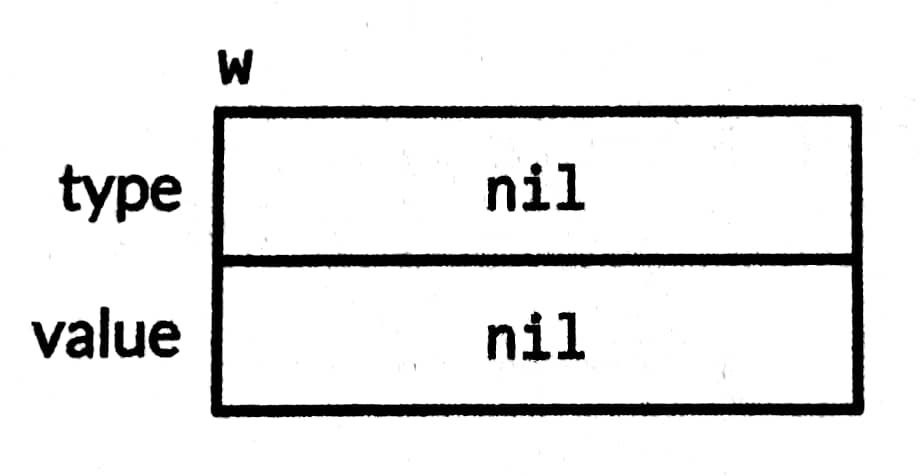
\includegraphics[width=0.4\linewidth]{figures/figura6.1}
\end{center}

Un valore interfaccia è descritto come nil o non-nil a seconda del suo tipo dinamico.

La seconda istruzione assegna un valore di tipo \verb|*os.File| a \verb|w|:
\begin{lstlisting}[frame=single, label={lst:lstlisting6-5.3}]
w = os.Stdout
\end{lstlisting}
Questo assegnamento coinvolge una conversione implicita da un tipo concreto al tipo di interfaccia, ed è equivalente alla conversione esplicita \verb|io.Writer(os.Stdout)|.
Una conversione di questo tipo cattura il tipo e il valore dei suoi operandi.
Il tipo dinamico del valore di interfaccia è impostato al descrittore del tipo per un tipo puntatore \verb|*os.File|, e il suo valore dinamico detiene una copia di \verb|os.Stdout|, che è un puntatore ad una variabile \verb|os.File| rappresentante lo standard output di un processo.
\begin{center}
    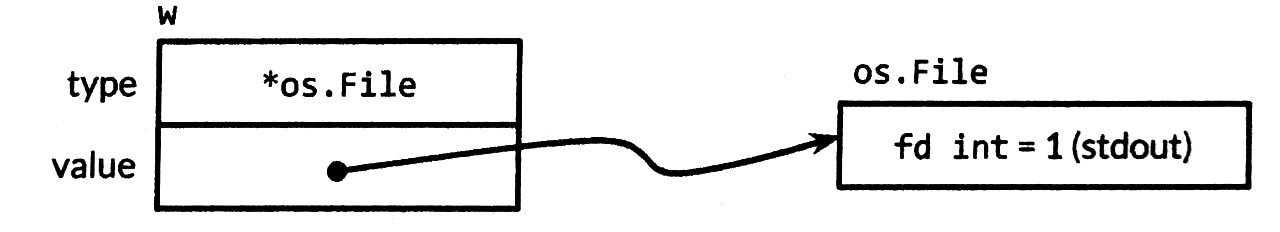
\includegraphics[width=0.5\linewidth]{figures/figura6.2}
\end{center}

In generale, non è possibile conoscere a compile-time quale tipo dinamico del valore di interfaccia sarà, così una chiamata tramite un interfaccia deve usare un \textit{invio dinamico}.
Invece di una chiamata diretta, il compilatore deve generare codice per ottenere l'indirizzo del metodo \verb|Write| dal tipo del descrittore, quindi produrre una chiamata indiretta a quel indirizzo.
L'argomento ricevitore per la chiamata è una copia del valore dinamico dell'interfaccia, \verb|os.Stdout|.
L'effetto è come se si fosse prodotta una chiamata direttamente.

La terza istruzione assegna un valore di tipo \verb|*bytes.Buffer| al valore di interfaccia:
\begin{lstlisting}[frame=single, label={lst:lstlisting6-5.4}]
w = new(bytes.Buffer)
\end{lstlisting}
Il tipo dinamico è ora \verb|*bytes.Buffer| e il valore dinamico è un puntatore al nuovo buffer allocato.
\begin{center}
    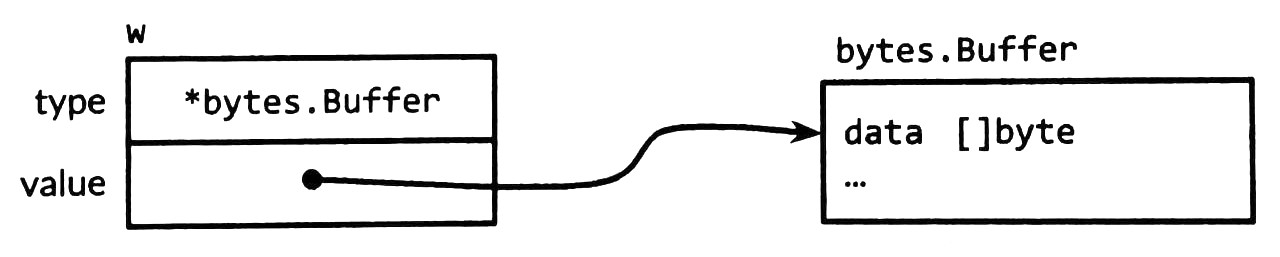
\includegraphics[width=0.5\linewidth]{figures/figura6.3}
\end{center}

Infine, la quarta istruzione assegna \verb|nil| al valore di interfaccia:
\begin{lstlisting}[frame=single, label={lst:lstlisting6-5.5}]
w = nil
\end{lstlisting}
Questo fa il reset di entrambi i suoi componenti a \verb|nil|, ripristinando \verb|w| allo stato della sua dichiarazione.

I valori di interfaccia possono essere confrontati usando \verb|==| e \verb|!=|, quindi utilizzabili anche come chiavi per le map o come gli operandi di un'istruzione switch.
Bisogna comunque fare attenzione, perché se le interfacce hanno stessi tipi dinamici, ma non confrontabili tra loro, allora il confronto fallisce con il lancio di un panic.
\begin{lstlisting}[frame=single, label={lst:lstlisting6-5.6}]
var x interface{} = []int{1, 2, 3}
fmt.Println(x == x) // panic: i tipi []int non sono
                    // confrontabili
\end{lstlisting}
Per questi motivi in generale si possono confrontare i valori di un interfaccia se si è certi che questo contenga valori dinamici di tipi confrontabili.


\section{L'interfaccia error}
\label{sec:interfaccia_error}%
Il tipo predichiarato \verb|error| è un tipo interfaccia con un singolo metodo che restituisce un messaggio d'errore:
\begin{lstlisting}[frame=single, label={lst:lstlisting6-6.1}]
type error interface {
    Error() string
}
\end{lstlisting}
Il modo più semplice per creare un \verb|error| è invocando \verb|errors.New|, che restituisce un nuovo \verb|error| per un dato messaggio d'errore.
L'intero package \verb|errors| è lungo solo 4 righe:
\begin{lstlisting}[frame=single, label={lst:lstlisting6-6.2}]
package errors

func New(text string) error { return &errorString{text} }

type errorString struct { text string }

func (e *errorString) Error() string { return e.text }
\end{lstlisting}
Il sottotipo di \verb|errorString| è una struct, non una stringa, a proteggere una sua rappresentazione da un aggiornamento involontario.
La ragione per cui il puntatore al tipo \verb|*errorString| soddisfa l'interfaccia \verb|error| è perché si vuole che ogni chiamata a \verb|New| allochi un'istanza distinta di \verb|error| diversa da tutte le altre.

Le chiamate a \verb|errors.New| sono relativamente poco frequenti perché esiste una funzione wrapper più conveniente, \verb|fmt.Errorf|, che permette pure la formattazione delle stringhe.